\part{Práctica 4}
\section{Actividad 4-1}
\label{p41}
\begin{center}
    \parbox{12cm}{\justify\textit{Escoja una de las bases de datos de clasificación para el trabajo de las dispuestas en Moodle (Breast Cancer, Dermatology, Fantasmas, Glass, Vehicle, Wine, Zoo). \\
    Se entiende que además de pasarla a formato .arff ya ha aplicado el preprocesamiento necesario en función del fichero ``\textbf{Pistas sobre los datasets con posible preprocesamiento a simple vista.pdf}'', en el caso de que sea una de las bases de datos que lo requiera.
    \begin{itemize}
        \item Cargue la base de datos y ejecute el algoritmo \textbf{C4.5} usando un 75\% para entrenar y un 25\% para generalizar, con los parámetros por defecto.
        \item Analice y muestre el árbol obtenido con los parámetros por defecto: nodo principal, número de nodos u hojas, variables presentes y omitidas. Comente también los resultados de las métricas obtenidas.
    \end{itemize}
    }}
\end{center}

Para la realización de esta actividad se va a utilizar la misma base de datos preprocesada de la práctica 3 (fantasmas). El objetivo es construir en Weka un árbol de decisión mediante el algoritmo C4.5, para lo cuál utilizaremos el clasificador llamado ``J48'' en Weka. Tal como indica el enunciado, se divide el conjunto en dos, seleccionando un 75\% (278 patrones) para la construcción del árbol (train) y el 25\%restante (93 patrones) para generalización (test). Weka realiza esta división manteniendo idénticas frecuencias de las clases en cada subconjunto.

El algoritmo construye el árbol mediante un proceso recursivo en el que, para establecer cada nodo se busca el atributo con mayor porcentaje de ganancia de información ($I(C,X_i)/H(X_i)$), generando una partición en dos del conjunto de datos. En caso de que el atributo sea continuo, el algoritmo es capaz de determinar el mejor umbral. Para cada división del conjunto se añade una arista desde el nodo generado y se repite el proceso con el subconjunto correspondiente. Cuando todos los patrones asociados aun determinado recorrido en profundidad tienen la misma clase, se añade un nodo hoja. El algoritmo C4.5 también permite realizar podas que o bien sustituyen un sub-árbol por un nodo hoja o bien por una parte éste (elevación de sub-árbol). Es interesante mencionar que con este algoritmo, a diferencia de C3, sí que podemos encontrar varias veces el mismo atributo al realizar un recorrido del árbol en profundidad, al menos en el caso de atributos continuos y con diferentes umbrales.

Tal como podemos observar en la figura \ref{fig:j48-arbol}, en este caso de estudio, el atributo de mayor ganancia es hair\_length, por tanto se establece como nodo raíz. El árbol generado cuenta con 53 nodos, 27 de los cuáles son nodos hoja. Cada nodo hoja indica la cantidad de patrones que, siendo de la clase indicada, han alcanzado el nodo así como la cantidad de patrones de otras clases que lo han alcanzado, en caso de haber alguno. Los nodos hoja muestran los resultados para todos los patrones, tanto de generalización como de entrenamiento.

\begin{landscape}
    \begin{figure}[H]
        \centering
        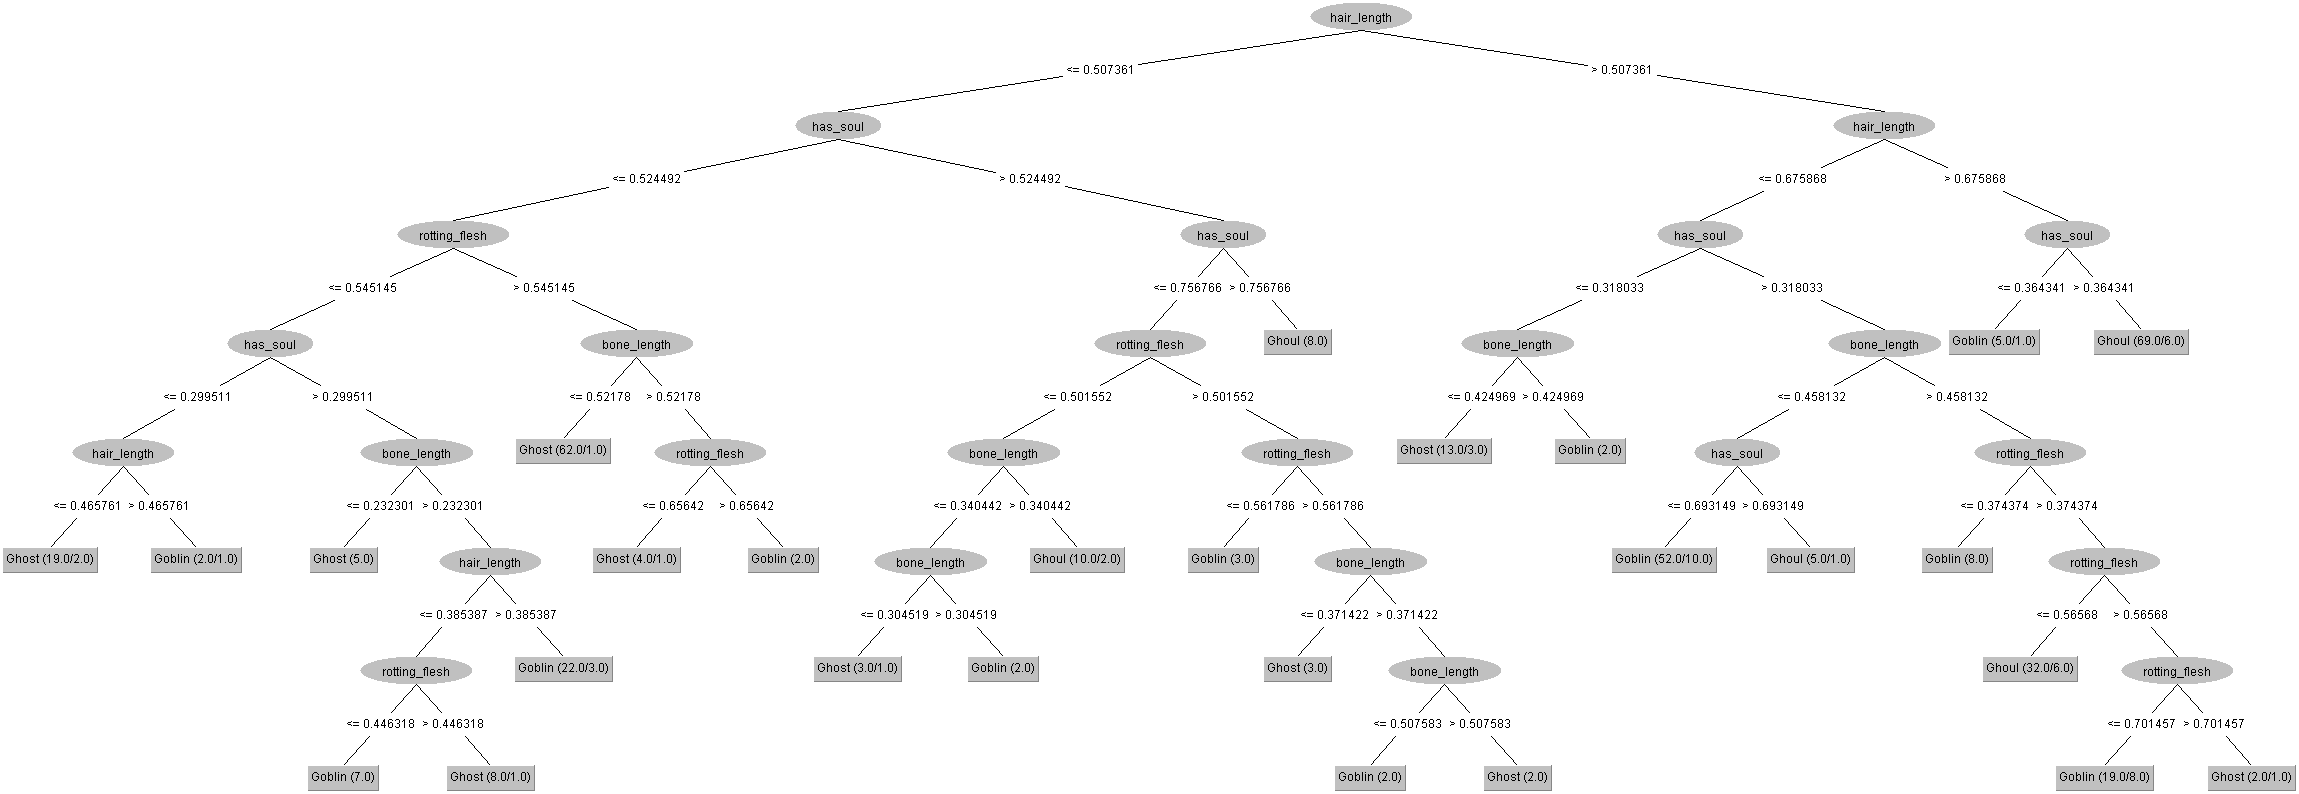
\includegraphics[height=0.5\textheight]{arbol}
        \caption{Árbol de decisión obtenido mediante C4.5}
        \label{fig:j48-arbol}
    \end{figure}
\end{landscape}

De los resultados del clasificador (fig. \ref{fig:j48-resultados}) podemos comentar que se han clasificado correctamente 65 patrones (69,89\%) de un total de 93 del conjunto de generalización. El estadístico Kappa es $\kappa=0,5473$, comparable aunque peor que el obtenido en los ensayos con otros tipos de clasificadores para el mismo conjunto de datos. La clase que peor se reconoce es de nuevo Goblin, con un TP Rate de 0,618, más elevado que el obtenido en los clasificadores anteriores, aunque hay que observar que en este caso, el FP Rate también es más alto, lo que da el peor resultado en AUC para todos los clasificadores utilizados con este conjunto. Esta comparación no es del todo justa porque se ha utilizado una técnica distinta para la generalización. En la matriz de confusión podemos ver que sólo 21 de los 34 Goblins han sido correctamente clasificados.
    
\begin{figure}[H]
    \centering
    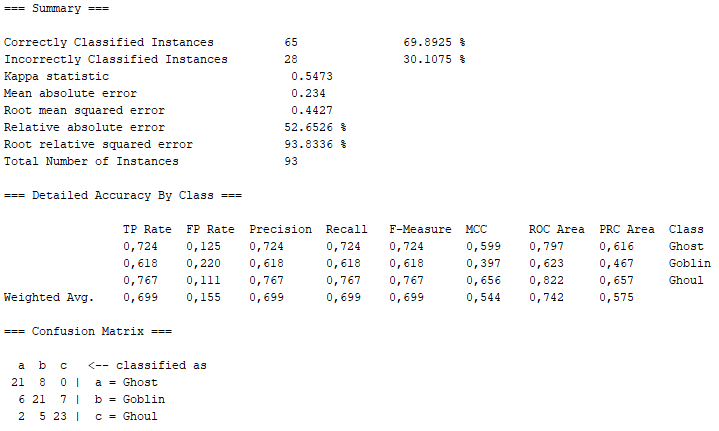
\includegraphics[width=\textwidth,keepaspectratio=true]{j48-resultados}
    \caption{Resultados del clasificador }
    \label{fig:j48-resultados}
\end{figure}


\clearpage
\section{Actividad 4-2}
\label{p42}
\begin{center}
    \parbox{12cm}{\justify\textit{Escoja una de las bases de datos de clasificación para el trabajo de las dispuestas en Moodle (Breast Cancer, Dermatology, Fantasmas, Glass, Vehicle, Wine, Zoo). \\
    Se entiende que además de pasarla a formato .arff ya ha aplicado el preprocesamiento necesario en función del fichero ``\textbf{Pistas sobre los datasets con posible preprocesamiento a simple vista.pdf}'', en el caso de que sea una de las bases de datos que lo requiera.
    \begin{itemize}
        \item Cargue la base de datos con un 75/25\% y ejecute el algoritmo Multilayer-Perceptron con los valores por defecto.
        \item ¿Qué observa al ir modificando sólo el \textbf{TrainingTime}? ¿Cambia el valor de Correctly Classified instances al modificar el parámetro? ¿Se estanca el aprendizaje o sobreentrena?
        \item ¿Qué observa al ir modificando sólo el \textbf{LearningRate}? ¿Cambia el valor de Correctly Classified instances al modificar el parámetro? ¿Se estanca el aprendizaje o sobreentrena?
    \end{itemize}
    }}
\end{center}

Para este ejercicio se utilizará el mismo conjunto de datos preprocesado (fantasmas) que en el ejercicio anterior. La partición del conjunto se realizará al 75/25\% tal como indica el enunciado, por lo que dispondremos de un conjunto de entrenamiento de 278 patrones y un conjunto de generalización de 93 con las mismas frecuencias de clases. El perceptrón tendrá tantos nodos en la capa de entrada como atributos la base de datos y tantos nodos en la capa de salida como valores puede tomar la clase (ver fig. \ref{fig:mlp-red}). Tanto el número de capas ocultas como el número de nodos en cada una de ellas es configurable, como veremos más adelante.

\begin{figure}[ht]
    \centering
    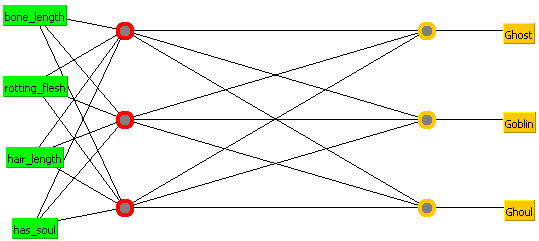
\includegraphics[width=\textwidth,keepaspectratio=true]{mlp-red}
    \caption{Topología de la red}
    \label{fig:mlp-red}
\end{figure}

A continuación repasaremos los parámetros de configuración más importantes y sus valores por defecto\footnote{En la captura se ha modificado el valor de GUI a true para poder capturar el diagrama de la red.} en MultilayerPerceptron (fig. \ref{fig:mlp-configuracion}). 
\begin{itemize}
    \item El parámetro hiddenLayers establece la configuración topológica de la red, en este caso, una única capa oculta con ``a'' nodos, donde el comodín ``a'' toma el valor del punto medio entre el número de atributos independientes y el número de clases. Para nuestro caso, $(3+3/2)=3$ nodos (ver fig. \ref{fig:mlp-red}).
    \item El parámetro learningRate o tasa de aprendizaje indica cuánto se modifican los pesos de las aristas durante el aprendizaje y viene a 0,3.
    \item El parámetro decay a false indica que el factor de aprendizaje se mantendrá constante a lo largo del aprendizaje.
    \item El parámetro momentum representa una especie de inercia que nos permite salir de un mínimo local, y toma valor por defecto 0,2. 
    \item  El parámetro trainingTime indica el número de épocas de entrenamiento, donde una época consiste en la evaluación de un patrón del conjunto de entrenamiento y el posterior ajuste de los pesos de la red mediante back propagation.
    \item El parámetro validationThreshold indica un número de épocas tal que, si el error de validación sube durante más épocas que las indicadas en el umbral, el aprendizaje se para aunque no se haya alcanzado el trainingTime. En el caso por defecto, este umbral se fija a 20 épocas.
\end{itemize}


\begin{figure}[ht]
    \centering
    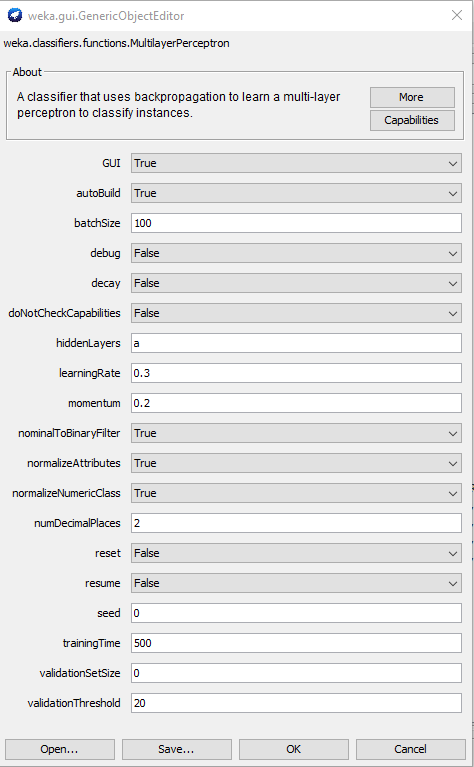
\includegraphics[width=.5\textwidth,keepaspectratio=true]{mlp-configuracion}
    \caption{Formulario de configuración para MultilayerPerceptron}
    \label{fig:mlp-configuracion}
\end{figure}

Al ejecutar el algoritmo con los valores por defecto, observamos unos resultados (ver fig. \ref{fig:mlp-resultados}) casi idénticos a los que se obtuvieron con J48 (ver fig. \ref{fig:j48-resultados}). $CCR=69,89\%$, 65 patrones correctamente clasificados frente a 28 incorrectamente clasificados, $\kappa=0,5455$, peor TP Rate para la clase Goblin con un valor de 0,676 y 23 goblins correctamente clasificados de 34. Dos más que con J48, aunque hay dos ghouls mal clasificados más y los mismos ghost, de ahí la coincidencia del CCR.


\begin{figure}[H]
    \centering
    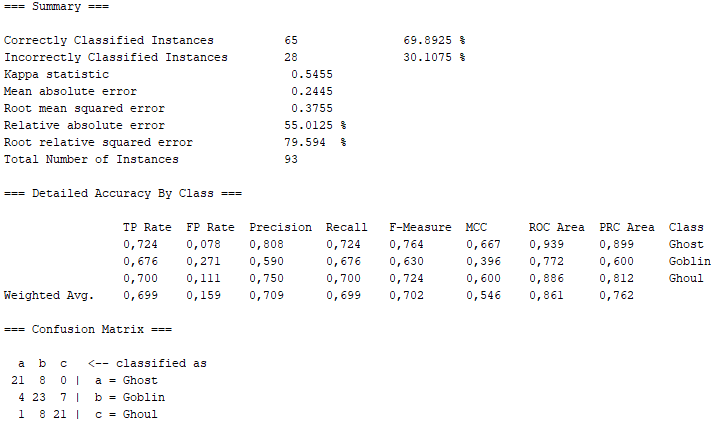
\includegraphics[width=\textwidth]{mlp-resultados}
    \caption{Resultados de MultilayerPerceptron con configuración por defecto}
    \label{fig:mlp-resultados}
\end{figure}

A continuación vamos a comprobar cómo afectan a los resultados las variaciones en el parámetro trainingTime. Para ello vamos a ejecutar el algoritmo variando dicho parámetro y tomaremos como medida de la bondad del resultado el número de patrones bien clasificados. Los datos obtenidos se muestran en el cuadro \ref{cuadro:variaciones-training-time}, donde se presenta el número de patrones correctamente clasificados (PCC) en función del valor de training time utilizado.

\begin{table}[ht]
    \centering
    \begin{tabular}{|r|c|c|c|c|c|c|c|c|c|c|c|c|}
    \hline
    \cellcolor[HTML]{9B9B9B}{\color[HTML]{FFFFFF} Training Time} & 5 & 10 & 50  & 100 & 200 & 300 & 400 & 500 & 1000 & 2000 & 5000  \\ \hline
    \cellcolor[HTML]{9B9B9B}{\color[HTML]{FFFFFF} PCC} & 67 & 66 & 64 & 64 & 64 & 64 & 65 & 65 & 66 & 65 & 64 \\ \hline
    \end{tabular}
    \caption{Patrones correctamente clasificados en función del training time}
    \label{cuadro:variaciones-training-time}
\end{table}

Aunque las variaciones son pequeñas dado que se trata de un conjunto pequeño, a la vista de los datos obtenidos, se deduce que existe un mínimo muy cerca de los pesos iniciales, que se alcanza a las pocas iteraciones pero del que sale también muy pronto, presumiblemente debido al momentum. A partir de las 10 épocas, el proceso está aparentemente estancado aunque mejora poco a poco hasta decaer de nuevo a partir de las 2000. Podría decirse que vemos sobre-entrenamiento a partir de la época 10, ya que el resultado empeora aunque habiendo entrenado tan poco ya es una casualidad.

Finalmente realizaremos un estudio similar al anterior pero esta vez manteniendo el valor por defecto de trainingTime y variando learningRate. De nuevo tomaremos como medida de bondad el número de patrones bien clasificados. Los datos obtenidos se muestran en el cuadro \ref{cuadro:variaciones-learning-rate}.

\begin{table}[ht]
    \centering
    \begin{tabular}{|r|c|c|c|c|c|c|c|}
    \hline
    \cellcolor[HTML]{9B9B9B}{\color[HTML]{FFFFFF} Learning Rate} & 0,05  & 0,1 & 0,2 & 0,3 & 0,4 & 0,5 & 1 \\ \hline
    \cellcolor[HTML]{9B9B9B}{\color[HTML]{FFFFFF} PCC} & 67 & 66 & 66 & 65 & 64 & 62 & 64 \\ \hline
    \end{tabular}
    \caption{Patrones correctamente clasificados en función del learning rate}
    \label{cuadro:variaciones-learning-rate}
\end{table}

Si antes cambiábamos el número de pasos, ahora cambiamos el tamaño de éstos, y los datos vienen a confirmar lo que se observó en el experimento anterior, ya que con un learningRate extremadamente pequeño alcanzamos un mínimo local que debe estar cercano al punto de partida. Según aumenta el learning rate empeora. Se podría decir que a partir de cierto learning-rate, un salto eventualmente nos hace salir del valle de la función de coste. Según aumenta el learning rate, los saltos son tan grandes que el resultado puede tanto mejorar como empeorar de época en época, y el aprendizaje deja de ser dirigido para volverse aleatorio.